\shorthandoff{:}
\newcommand{\Etape}[2]{
\node[Etape,label={right:#2}] (#1) {};
}
\newcommand{\EtapeLink}[3]{
\node[Etape,below of=#3,label={[align=left]right:#2}] (#1) {};
\draw[->] (#3) -- (#1);
}
\newcommand{\TransLink}[3]{
\node[Trans,align=center,below of=#3] (#1) {};
\node[align=center,anchor=west,at =(#1.east),xshift=10pt] {#2};
\draw[->] (#3) -- (#1);
}
\newcommand{\TransActionLink}[3]{
\node[Trans,align=center,below of=#3] (#1) {};
\node[Line,align=center,anchor=west,at =(#1.east),xshift=10pt] {#2};
\draw[->] (#3) -- (#1);
}



	\tikzset{every node/.style={font=\small, node distance =  0.6cm}}
	\tikzset{Etape/.style={draw,black,minimum size=0.6cm,inner sep=0pt,circle,font=\tiny}}
	\tikzset{Trans/.style={draw,black,minimum width=0.6cm,minimum height=0.0cm,inner sep=0pt,outer sep=0pt,rectangle,font=\tiny}}
	
	%\tikzset{Line/.style={path picture={\draw[black] (path picture bounding box.north west) -- (path picture bounding box.north east);}}}
	\tikzset{Line/.style={path picture={\draw[black] (path picture bounding box.west) -- (path picture bounding box.east);}}}

\begin{tikzpicture}
\Etape{I}{$T_x:=Bit_{Stop}$}
\TransLink{T1}{Volonté d'envoyer}{I}
\EtapeLink{S}{$T_x:=Bit_{Start}$}{T1}
\TransActionLink{T2}{$\uparrow$ I$_{clk}$ \\ $i:=8$}{S}
\EtapeLink{D}{\emph{Bit de donnée}}{T2}
%\tikzstyle{every label}={draw,red,font=\tiny}

\node[Trans,node distance = 1.5cm,left of=D] (T) {};
\node[Line,align=center,anchor=east,at =(T.west),xshift=-10pt] (V) {$\uparrow$ I$_{clk}$ $\cdot$ $i>0$\\[1em]$T_x:=T_{Data}[i]$, $i$-\,- };
\draw[->] (D) edge [out=225,in=-90] (T);
\draw[->] (T) edge [out=90,in=135] (D);

\TransLink{T3}{$\uparrow$ I$_{clk}$ $\cdot$ $i=0$}{D}
\EtapeLink{S}{$T_x:=Bit_{Stop}$}{T3}
\TransActionLink{T4}{$\uparrow$ I$_{clk}$ \\ /Fin Transmition}{S}

\draw[-] (T4) edge [out=-90,in=-90] ($(V.west)-(10pt,0)$);
\draw[->] ($(V.west)-(10pt,0)$) edge [out=90] (I);
\end{tikzpicture}

% reception des données

\begin{tikzpicture}%[every node/.style={font=\tiny}]
\Etape{I}{Attente}
\TransActionLink{T1}{$\uparrow$ I$_{clk}$ $\cdot$ $R_x=Bit_{Start}$ \\ $i:=8$ }{I}
\EtapeLink{D}{\emph{Bit de donnée}}{T1}
%\tikzstyle{every label}={draw,red,font=\tiny}

\node[Trans,node distance = 1.5cm,left of=D] (T) {};
\node[Line,align=center,anchor=east,at =(T.west),xshift=-10pt] (V) {$\uparrow$ I$_{clk}$ $\cdot$ $i>0$\\[1em]$R_{Data}[i]:=R_x$, $i$-\,- };
\draw[->] (D) edge [out=225,in=-90] (T);
\draw[->] (T) edge [out=90,in=135] (D);

\TransLink{T3}{$\uparrow$ I$_{clk}$ $\cdot$ $i=0$}{D}
\EtapeLink{S}{Attente}{T3}
\TransActionLink{T4}{$R_x=Bit_{Stop}$\\ /Fin Réception}{S}

\draw[-] (T4) edge [out=-90,in=-90] ($(V.west)-(10pt,0)$);
\draw[->] ($(V.west)-(10pt,0)$) edge [out=90] (I);
\end{tikzpicture}

% Schema de communication

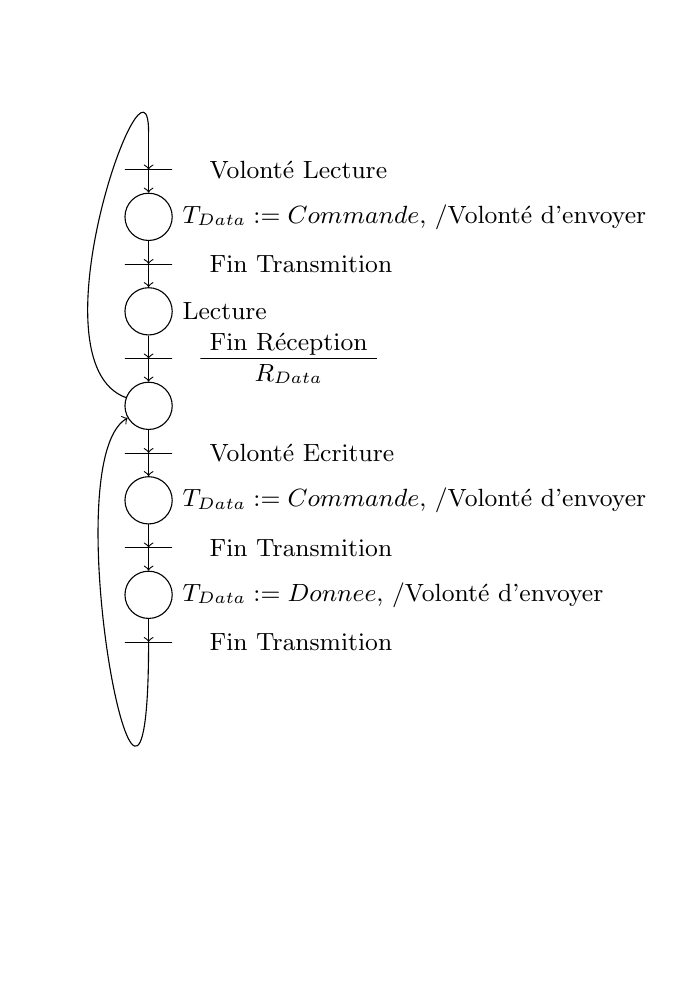
\begin{tikzpicture}%[every node/.style={font=\tiny}]

\node (T) {};

\TransLink{T1}{Volonté Lecture}{T}

\EtapeLink{E1}{$T_{Data}:=Commande$, /Volonté d'envoyer}{T1}

\TransLink{T2}{Fin Transmition}{E1}

\EtapeLink{E2}{Lecture}{T2}

\TransActionLink{T3}{Fin Réception \\ $R_{Data}$}{E2}

\EtapeLink{E3}{}{T3}

	\draw[-] (E3) edge [out=160, in=90] (T.south);


\TransLink{T1}{Volonté Ecriture}{E3}

\EtapeLink{E1}{$T_{Data}:=Commande$, /Volonté d'envoyer}{T1}

\TransLink{T2}{Fin Transmition}{E1}

\EtapeLink{E2}{$T_{Data}:=Donnee$, /Volonté d'envoyer}{T2}

\TransLink{T3}{Fin Transmition}{E2}

	\draw[->] (T3) edge [out=-90, in=210,out distance=4cm] (E3);

\end{tikzpicture}
